% Provenance (never printed): BCPST year 1 geology (2021), "la carte
% geologique" (reading a map, structures, chronology), union licence
% Sciences de la Terre L1 (cartographie: strike and dip, three-point problem,
% outcrop patterns, DEM and GIS). See sources/outline_sources.md. Pilot
% chapter, 2026-10-22. The region is the series' invented Varden Hills
% (figdata/shared/region.py); every number about it is computed in
% figdata/bachelor-1/varden_maps.py or figdata/bachelor-1/v_rule.py.
\chapter{Peta geologi}\label{ch:b1:geological-maps}

Seorang ahli geologi melintasi deretan bukit rendah dengan papan peta, buku catatan, dan kompas-klinometer. Sebagian besar tanahnya berumput, berhutan, atau ladang yang dibajak; batuan hanya tampak di sana-sini, di tepi aliran kecil, di potongan jalan, di tebing. Dari kilasan-kilasan yang tersebar itu, dan dari bentuk permukaan tanah, ahli geologi harus menyatakan batuan apa yang berada di bawah setiap meter persegi bukit-bukit itu, bagaimana lapisannya miring, di mana ia patah, dan dalam urutan apa semua itu terjadi. Hasilnya adalah \omterm{def:b1:geological-maps:geological-map}{peta geologi}: gambar datar yang menyandi sebuah tubuh batuan tiga dimensi. Bab ini menjelaskan bagaimana peta seperti itu dibuat dan dibaca --- bagaimana \omterm{def:b1:geological-maps:attitude}{orientasi} suatu permukaan diukur dan dihitung, mengapa \omterm{def:b1:geological-maps:geological-map}{singkapan} suatu lapisan membentuk pola yang demikian, dan bagaimana sebuah peta menceritakan sejarah. Contohnya diambil dari wilayah khayal tetapi konsisten secara geologi, Perbukitan Varden, yang muncul berulang kali dalam buku ini.

\begin{recall}
Peta topografi memperlihatkan relief dengan garis kontur, yaitu garis elevasi yang sama; skalanya menghubungkan jarak pada peta dengan jarak di lapangan (Buku 1, kelas 9). Umur relatif mengikuti dari superposisi (suatu lapisan lebih muda daripada lapisan di bawahnya, kecuali urutannya telah terbalik), dari pemotongan silang (apa pun yang memotong batuan lebih muda daripadanya) dan dari inklusi (Buku 1, kelas 7). Sesar adalah rekahan sepanjang mana dua blok telah bergeser (Buku 1, kelas 7); geometri \omterm{def:b1:geological-maps:fold}{lipatan} dan sesar menjadi pokok bahasan \cref{ch:b1:faults-folds-fabrics}.
\end{recall}

\section{Peta adalah irisan dari tiga dimensi}\label{sec:b1:geological-maps:cut}

\begin{definition}[Peta geologi]\label{def:b1:geological-maps:geological-map}
Sebuah \emph{peta geologi}\index{peta geologi} memperlihatkan, di setiap titik permukaan tanah, satuan batuan yang berada di sana di bawah tanah, dengan \emph{kontak}\index{kontak (geologi)} --- permukaan yang memisahkan dua satuan --- dan struktur (sesar, \omterm{def:b1:geological-maps:fold}{sumbu lipatan}, \omterm{def:b1:geological-maps:attitude}{orientasi} lapisan) yang memengaruhinya. Sebuah \emph{satuan peta}\index{satuan peta} adalah tubuh batuan yang dapat dikenali dan diikuti di lapangan serta digambar dalam satu warna; \emph{singkapannya}\index{singkapan} adalah area tempat ia berada di permukaan.
\end{definition}

\begin{definition}[Model elevasi digital]\label{def:b1:geological-maps:dem}
Yang disebut \emph{model elevasi digital}\index{model elevasi digital} adalah kisi elevasi tanah, $z = g(x,y)$, pada titik-titik yang berjarak teratur. Sistem informasi geografis menyimpan kisi-kisi semacam itu dan lapisan-lapisan lain peta (\omterm{def:b1:geological-maps:geological-map}{kontak}, sesar, pengukuran, lubang bor) dalam satu kerangka koordinat bersama, serta menghitung dengan mereka.
\end{definition}

\begin{proposition}[Singkapan suatu kontak]\label{prop:b1:geological-maps:intersection}
Misalkan permukaan tanah adalah permukaan $z = g(x,y)$ dan sebuah \omterm{def:b1:geological-maps:geological-map}{kontak} adalah permukaan
$z = c(x,y)$. Jejak \omterm{def:b1:geological-maps:geological-map}{kontak} pada peta adalah kurva
\[
  g(x,y) = c(x,y),
\]
yaitu proyeksi pada bidang horizontal dari perpotongan kedua permukaan itu. Satuan yang berada di atas \omterm{def:b1:geological-maps:geological-map}{kontak} tersingkap di tempat $g > c$.
\end{proposition}

\begin{proof}
Sebuah titik pada peta berada pada jejak jika dan hanya jika permukaan tanah di titik itu termasuk \omterm{def:b1:geological-maps:geological-map}{kontak}, yaitu $g(x,y) = c(x,y)$. Di tempat $g(x,y) > c(x,y)$, tanah berada di atas \omterm{def:b1:geological-maps:geological-map}{kontak}: batuan di permukaan termasuk satuan yang berada di atasnya.
\end{proof}

\begin{remark}[Cara peta-peta buku ini digambar]\label{rem:b1:geological-maps:computed}
Inilah tepatnya cara sebuah sistem informasi geografis menggambar peta dari model tiga dimensi: ia menghitung $g - c$ pada kisi \omterm{def:b1:geological-maps:dem}{model elevasi digital} dan menelusuri kurva tempat tanda itu berubah. Peta Perbukitan Varden dalam buku ini digambar dengan cara itu, dari model geologi yang setiap permukaannya diketahui.
\end{remark}

\begin{omfigure}
\begin{tikzpicture}
\begin{axis}[axis equal image, xmin=0, xmax=10, ymin=0, ymax=8, width=0.82\linewidth,
  tick label style={font=\scriptsize}, xlabel={timur (km)}, ylabel={utara (km)},
  label style={font=\small}, colormap/blackwhite, enlargelimits=false]
\addplot[matrix plot*, mesh/cols=101, point meta=explicit, shader=interp] table[x=x_km, y=y_km, meta=shade] {figdata/out/bachelor-1-varden_maps-shade.dat};
\addplot[contour, line width=0.25pt, opacity=0.7] table {figdata/out/shared-region-contours.dat};
\addplot[index contour, opacity=0.8] table {figdata/out/shared-region-index-contours.dat};
\addplot[river] table {figdata/out/shared-region-river.dat};
\end{axis}
\end{tikzpicture}

{\small Perbukitan Varden sebagai \omterm{def:b1:geological-maps:dem}{model elevasi digital}: tanah diterangi dari barat laut, dengan kontur setiap \qty{50}{m} (lebih tebal pada 250 dan \qty{500}{m}) dan sungai, yang mengalir ke timur.}
\end{omfigure}

\begin{omfigure}
\begin{tikzpicture}
\begin{axis}[axis equal image, xmin=0, xmax=10, ymin=0, ymax=8, width=0.82\linewidth,
  tick label style={font=\scriptsize}, xlabel={timur (km)}, ylabel={utara (km)},
  label style={font=\small}]
\addplot[lith schist, draw=black, line width=0.3pt, even odd rule] table {figdata/out/shared-region-unit-schist.dat};
\addplot[lith granite, draw=black, line width=0.3pt, even odd rule] table {figdata/out/shared-region-unit-granite.dat};
\addplot[om lith={icsTriassic!35}{om sand}, draw=black, line width=0.3pt, even odd rule] table {figdata/out/shared-region-unit-sandstone.dat};
\addplot[om lith={icsJurassic!40}{om limestone}, draw=black, line width=0.3pt, even odd rule] table {figdata/out/shared-region-unit-limestone.dat};
\addplot[om lith={icsJurassic!15}{om shale}, draw=black, line width=0.3pt, even odd rule] table {figdata/out/shared-region-unit-shale.dat};
\addplot[om lith={icsCretaceous!35}{om limestone}, draw=black, line width=0.3pt, even odd rule] table {figdata/out/shared-region-unit-chalk.dat};
% the fault is drawn before the alluvium: the younger alluvial floor conceals it
\addplot[normal fault] table {figdata/out/shared-region-fault.dat};
\addplot[lith alluvium, draw=black, line width=0.3pt, even odd rule] table {figdata/out/shared-region-unit-alluvium.dat};
\addplot[contour, opacity=0.55] table {figdata/out/shared-region-contours.dat};
\addplot[river] table {figdata/out/shared-region-river.dat};
\pic at (axis cs:4.3,6.6) {strikedip={350.6}{12}};
\pic at (axis cs:2.2,6.6) {strikedip={189.3}{12}};
\pic at (axis cs:8.6,1.4) {northarrow};
\fill[black] (axis cs:6.6,0.35) rectangle (axis cs:7.1,0.5);
\fill[white] (axis cs:7.1,0.35) rectangle (axis cs:7.6,0.5);
\fill[black] (axis cs:7.6,0.35) rectangle (axis cs:8.1,0.5);
\fill[white] (axis cs:8.1,0.35) rectangle (axis cs:8.6,0.5);
\draw[black, line width=0.4pt] (axis cs:6.6,0.35) rectangle (axis cs:8.6,0.5);
\node[font=\footnotesize, above, inner sep=1.5pt, fill=white, fill opacity=0.8, text opacity=1] at (axis cs:7.6,0.5) {\qty{2}{km}};
\end{axis}
\end{tikzpicture}

\smallskip
\begin{tikzpicture}[font=\footnotesize]
\matrix[column sep=7pt, row sep=3pt, matrix of nodes, nodes={anchor=west}] {
  \tikz\draw[black!60, line width=0.4pt, lith alluvium] (0,0) rectangle (0.7,0.32); & aluvium (Kuarter) &
  \tikz\draw[black!60, line width=0.4pt, om lith={icsCretaceous!35}{om limestone}] (0,0) rectangle (0.7,0.32); & kapur (Kapur, 90 Ma) \\
  \tikz\draw[black!60, line width=0.4pt, om lith={icsJurassic!15}{om shale}] (0,0) rectangle (0.7,0.32); & serpih (Jura, 165 Ma) &
  \tikz\draw[black!60, line width=0.4pt, om lith={icsJurassic!40}{om limestone}] (0,0) rectangle (0.7,0.32); & batu gamping (Jura, 180 Ma) \\
  \tikz\draw[black!60, line width=0.4pt, om lith={icsTriassic!35}{om sand}] (0,0) rectangle (0.7,0.32); & batu pasir (Trias, 245 Ma) &
  \tikz\draw[black!60, line width=0.4pt, lith granite] (0,0) rectangle (0.7,0.32); & granit (310 Ma) \\
  \tikz\draw[black!60, line width=0.4pt, lith schist] (0,0) rectangle (0.7,0.32); & sekis (480 Ma) &
  \tikz\draw[normal fault] (0,0.16) -- (0.9,0.16); & sesar normal (tanda di sisi yang turun) \\
};
\end{tikzpicture}

{\small \omterm{def:b1:geological-maps:geological-map}{Peta geologi} Perbukitan Varden, dengan kontur, sungai, dua pengukuran \omterm{def:b1:geological-maps:attitude}{orientasi} (garis \omterm{def:b1:geological-maps:attitude}{jurus} dan tanda \omterm{def:b1:geological-maps:attitude}{kemiringan}, dengan \omterm{def:b1:geological-maps:attitude}{kemiringan} dalam derajat) dan legenda. Umur-umurnya adalah umur satuan-satuan wilayah itu; sesar tersembunyi di bawah aluvium muda dataran lembah.}
\end{omfigure}

\section{Orientasi sebuah bidang}

\begin{definition}[Jurus, kemiringan dan arah kemiringan]\label{def:b1:geological-maps:attitude}
Misalkan suatu permukaan geologi --- bidang perlapisan, \omterm{def:b1:geological-maps:geological-map}{kontak}, atau sesar --- secara lokal berupa bidang. \emph{Jurus}\index{jurus} adalah arah garis-garis horizontal yang dikandungnya, diberikan sebagai \omterm{def:b1:spherical-astronomy:horizontal}{azimut} (derajat searah jarum jam dari utara). \emph{Kemiringan}\index{kemiringan} $\delta$ adalah sudut antara bidang dan horizontal, diukur pada bidang vertikal yang tegak lurus jurus, $0 \le \delta \le \ang{90}$. \emph{Arah kemiringan}\index{arah kemiringan} $\alpha$ adalah \omterm{def:b1:spherical-astronomy:horizontal}{azimut} garis paling curam yang menurun pada bidang itu. Bersama-sama keduanya membentuk \emph{orientasi}\index{orientasi (bidang)} bidang itu, ditulis arah kemiringan/kemiringan, misalnya $080/12$.
\end{definition}

\begin{notation}[Jurus menurut kaidah tangan kanan]\label{not:b1:geological-maps:rhr}
Sebuah \omterm{def:b1:geological-maps:attitude}{jurus} dapat dibaca dalam dua arah yang berlawanan. \emph{Kaidah tangan kanan} memilih arah yang bidangnya miring ke kanan bagi pengamat yang melihat sepanjang \omterm{def:b1:geological-maps:attitude}{jurus}: \omterm{def:b1:geological-maps:attitude}{jurus} $= \alpha - \ang{90}$ (modulo \ang{360}). Pada peta, simbolnya adalah garis \omterm{def:b1:geological-maps:attitude}{jurus} dengan tanda pendek yang menunjuk ke bawah \omterm{def:b1:geological-maps:attitude}{kemiringan}, diberi label \omterm{def:b1:geological-maps:attitude}{kemiringannya}.
\end{notation}

\begin{omfigure}
\tdplotsetmaincoords{65}{125}
\begin{tikzpicture}[tdplot_main_coords, font=\small, scale=1.05]
  % the horizontal plane
  \fill[omSea!50] (-2.2,-1.6,0) -- (2.2,-1.6,0) -- (2.2,1.6,0) -- (-2.2,1.6,0) -- cycle;
  \draw[black!40] (-2.2,-1.6,0) -- (2.2,-1.6,0) -- (2.2,1.6,0) -- (-2.2,1.6,0) -- cycle;
  % the dipping plane: strike along y (north), dipping east (+x) at 30 degrees
  \fill[omLithLime!80, opacity=0.85] (-0.0,-1.6,0) -- (-0.0,1.6,0) -- (2.2,1.6,-1.27) -- (2.2,-1.6,-1.27) -- cycle;
  \draw[black!60] (0,-1.6,0) -- (0,1.6,0) -- (2.2,1.6,-1.27) -- (2.2,-1.6,-1.27) -- cycle;
  % strike line (horizontal, in both planes)
  \draw[omThm, line width=1.1pt] (0,-1.6,0) -- (0,1.6,0);
  % dip line and the horizontal below it, with the dip angle
  \draw[omDef, line width=1.1pt, -{Stealth[length=2.4mm]}] (0,0,0) -- (2.2,0,-1.27);
  \draw[black!60, densely dashed] (0,0,0) -- (2.2,0,0);
  \draw[black!60, densely dashed] (2.2,0,0) -- (2.2,0,-1.27);
  \draw[black] plot[domain=0:30, samples=16, variable=\t] ({0.8*cos(\t)}, 0, {-0.8*sin(\t)});
  \node[font=\footnotesize] at (1.05,0,-0.22) {$\delta$};
  % north arrow on the horizontal plane
  \draw[black, -{Stealth[length=2mm]}] (-1.8,-1.2,0) -- (-1.8,-0.3,0);
  \node[font=\footnotesize] at (-1.8,-0.05,0) {U};
\end{tikzpicture}
\begin{tikzpicture}[font=\small]
  \node[align=left, anchor=west, text width=5.2cm] at (0,0) {%
    \textcolor{omThm}{\rule[0.5ex]{0.6cm}{1.1pt}} jurus: garis horizontal bidang;\\[3pt]
    \textcolor{omDef}{\rule[0.5ex]{0.6cm}{1.1pt}} garis paling curam yang menurun pada bidang, yang azimutnya adalah arah kemiringan;\\[3pt]
    kemiringan adalah sudut antara garis ini dan horizontal (putus-putus).};
\end{tikzpicture}

{\small Sebuah bidang berjurus utara dan miring \ang{30} ke timur (\omterm{def:b1:geological-maps:attitude}{orientasi} $090/30$), memotong bidang horizontal sepanjang garis \omterm{def:b1:geological-maps:attitude}{jurusnya}. Tidak sesuai skala.}
\end{omfigure}

\begin{proposition}[Persamaan bidang miring]\label{prop:b1:geological-maps:plane}
Dengan $x$ ke timur, $y$ ke utara dan $z$ ke atas, bidang dengan \omterm{def:b1:geological-maps:attitude}{arah kemiringan} $\alpha$ dan \omterm{def:b1:geological-maps:attitude}{kemiringan} $\delta$ yang melalui titik $(x_0, y_0, z_0)$ adalah
\[
  z = z_0 - \tan\delta\,\bigl[(x - x_0)\sin\alpha + (y - y_0)\cos\alpha\bigr].
\]
\end{proposition}

\begin{proof}
Vektor satuan horizontal yang menunjuk ke \omterm{def:b1:geological-maps:attitude}{arah kemiringan} adalah
$\vec u = (\sin\alpha, \cos\alpha, 0)$ (\omterm{def:b1:spherical-astronomy:horizontal}{azimut} diukur dari utara, yaitu sumbu $y$, menuju timur, yaitu sumbu $x$). Sepanjang \omterm{def:b1:geological-maps:attitude}{jurus}, tegak lurus $\vec u$, bidang itu horizontal; sepanjang $\vec u$ ia turun sebesar $\tan\delta$ per satuan jarak horizontal. Jarak horizontal suatu titik dari garis \omterm{def:b1:geological-maps:attitude}{jurus} yang melalui $(x_0, y_0)$, dihitung positif ke \omterm{def:b1:geological-maps:attitude}{arah kemiringan}, adalah $(x-x_0)\sin\alpha + (y-y_0)\cos\alpha$, dari situlah rumusnya diperoleh.
\end{proof}

\begin{theorem}[Orientasi dari tiga titik]\label{thm:b1:geological-maps:three-point}
Misalkan $P_1, P_2, P_3$ tiga titik tak segaris pada suatu bidang, dan
$\vec n = \overrightarrow{P_1P_2} \times \overrightarrow{P_1P_3} =
(n_x, n_y, n_z)$, dipilih dengan $n_z > 0$ (ganti $\vec n$ dengan $-\vec n$
jika tidak). Maka \omterm{def:b1:geological-maps:attitude}{kemiringan} dan \omterm{def:b1:geological-maps:attitude}{arah kemiringan} bidang itu adalah
\[
  \delta = \arccos\frac{n_z}{\|\vec n\|}, \qquad
  \alpha = \text{azimut vektor horizontal } (n_x, n_y),
\]
yaitu sudut $\alpha \in [\ang{0}, \ang{360})$ dengan
$\sin\alpha = n_x/\sqrt{n_x^2+n_y^2}$ dan $\cos\alpha = n_y/\sqrt{n_x^2+n_y^2}$
(bidang horizontal jika $n_x = n_y = 0$).
\end{theorem}

\begin{proof}
$\vec n$ tegak lurus terhadap dua vektor yang bebas linear di dalam bidang, sehingga tegak lurus terhadap bidang itu. \omterm{def:b1:geological-maps:attitude}{Kemiringan} adalah sudut antara bidang dan horizontal, sama dengan sudut antara normal-normalnya, $\vec n$ dan vertikal $\vec k$: $\cos\delta = \vec n \cdot \vec k / \|\vec n\| = n_z/\|\vec n\|$.
Menurut \cref{prop:b1:geological-maps:plane}, bidang itu adalah $z = \text{konstanta} -
\tan\delta\,(x\sin\alpha + y\cos\alpha)$, yaitu
$\tan\delta\sin\alpha\,x + \tan\delta\cos\alpha\,y + z = \text{konstanta}$; normal ke atasnya sebanding dengan $(\tan\delta\sin\alpha,
\tan\delta\cos\alpha, 1)$, yang bagian horizontalnya menunjuk ke \omterm{def:b1:geological-maps:attitude}{arah kemiringan}
$\alpha$. Karena $\vec n$ adalah kelipatan positif dari normal ini, $(n_x, n_y)$
menunjuk ke \omterm{def:b1:geological-maps:attitude}{arah kemiringan} juga.
\end{proof}

\begin{method}[Masalah tiga titik]\label{met:b1:geological-maps:three-point}
Untuk mencari \omterm{def:b1:geological-maps:attitude}{orientasi} suatu \omterm{def:b1:geological-maps:geological-map}{kontak} yang ditemui di tiga lubang bor (atau terlihat di tiga \omterm{def:b1:geological-maps:geological-map}{singkapan}):
\begin{enumerate}
  \item untuk setiap lubang bor, ambil elevasi \omterm{def:b1:geological-maps:geological-map}{kontak} itu: elevasi tanah dikurangi kedalaman tempat \omterm{def:b1:geological-maps:geological-map}{kontak} ditemui;
  \item tulislah ketiga titik $P_i = (x_i, y_i, z_i)$ dalam meter, $x$ ke timur, $y$ ke utara;
  \item hitunglah $\vec n = \overrightarrow{P_1P_2} \times
        \overrightarrow{P_1P_3}$ dan buat $n_z$ positif;
  \item terapkan \cref{thm:b1:geological-maps:three-point}; nyatakan \omterm{def:b1:geological-maps:attitude}{orientasinya} sebagai \omterm{def:b1:geological-maps:attitude}{arah kemiringan}/\omterm{def:b1:geological-maps:attitude}{kemiringan} dan, jika diminta, \omterm{def:b1:geological-maps:attitude}{jurusnya} menurut kaidah tangan kanan.
\end{enumerate}
Di atas kertas, soal yang sama diselesaikan dengan kontur struktur: pada garis yang menghubungkan titik tertinggi dan terendah, carilah dengan perbandingan titik pada elevasi titik ketiga; garis yang melalui kedua titik dengan elevasi sama itu adalah garis \omterm{def:b1:geological-maps:attitude}{jurus}; \omterm{def:b1:geological-maps:attitude}{kemiringan} mengikuti dari selisih elevasi antara dua garis \omterm{def:b1:geological-maps:attitude}{jurus} sejajar dan jaraknya.
\end{method}

\begin{example}[Sayap timur antiklin Varden]\label{ex:b1:geological-maps:east}
% computed in figdata/bachelor-1/varden_maps.py (boreholes E1-E3)
Tiga lubang bor, E1 di $(4000, 6000)$, E2 di $(4600, 7200)$ dan E3 di $(5100, 6400)$ (meter ke timur dan utara dari sudut barat daya peta), menemui dasar batu gamping pada elevasi $174$, $4$ dan $\qty{-74}{m}$. Maka
$\overrightarrow{P_1P_2} = (600, 1200, -170)$,
$\overrightarrow{P_1P_3} = (1100, 400, -248)$; hasil kali silangnya adalah
$(-229\,600, -38\,200, -1\,080\,000)$, yang menunjuk ke bawah, sehingga
\[
  \vec n = (229\,600,\ 38\,200,\ 1\,080\,000).
\]
Maka $\cos\delta = 1\,080\,000/\|\vec n\| \approx
0.9776$, $\delta \approx \ang{12.2}$, dan \omterm{def:b1:geological-maps:attitude}{arah kemiringannya} adalah \omterm{def:b1:spherical-astronomy:horizontal}{azimut} dari
$(229\,600, 38\,200)$, $\alpha \approx \ang{80.6}$: \omterm{def:b1:geological-maps:attitude}{orientasinya} adalah
$081/12$, \omterm{def:b1:geological-maps:attitude}{jurus} $\ang{351}$ menurut kaidah tangan kanan. Dasar batu gamping itu miring landai ke timur-timur laut.
\end{example}

\section{Pola singkapan}

\begin{proposition}[Kontak horizontal dan vertikal]\label{prop:b1:geological-maps:hv}
Jejak \omterm{def:b1:geological-maps:geological-map}{kontak} horizontal mengikuti garis kontur dengan elevasinya. Jejak \omterm{def:b1:geological-maps:geological-map}{kontak} vertikal adalah garis lurus pada peta, apa pun reliefnya.
\end{proposition}

\begin{proof}
Untuk $c(x,y) = z_0$, jejak $g(x,y) = z_0$ adalah kontur $z_0$
(\cref{prop:b1:geological-maps:intersection}). Bidang vertikal adalah himpunan titik yang posisi horizontalnya terletak pada satu garis lurus, pada elevasi mana pun; jejaknya pada peta adalah garis itu.
\end{proof}

\begin{theorem}[Aturan-V]\label{thm:b1:geological-maps:v-rule}
\omterm{def:b1:geological-maps:geological-map}{Kontak} planar memotong lembah yang dasarnya menurun ke hilir dengan gradien $s > 0$. Misalkan $a$ tangen \omterm{def:b1:geological-maps:attitude}{kemiringan} semu \omterm{def:b1:geological-maps:geological-map}{kontak} itu ke arah hilir ($a > 0$ bila miring ke hilir, $a < 0$ bila miring ke hulu, $a = 0$ bila horizontal). Maka jejak \omterm{def:b1:geological-maps:geological-map}{singkapannya} membentuk huruf V yang puncaknya terletak pada dasar lembah, dan
\begin{itemize}
  \item menunjuk ke \emph{hilir} bila $a > s$: \omterm{def:b1:geological-maps:geological-map}{kontak} miring ke hilir lebih curam daripada dasar lembah menurun;
  \item menunjuk ke \emph{hulu} bila $a < s$: \omterm{def:b1:geological-maps:geological-map}{kontak} horizontal, miring ke hulu, atau miring ke hilir lebih landai daripada dasar.
\end{itemize}
\omterm{def:b1:geological-maps:geological-map}{Kontak} vertikal tidak membentuk V.
\end{theorem}

\begin{proof}
Misalkan $\xi$ jarak yang diukur ke hilir sepanjang dasar lembah. Dasar itu berada pada elevasi $z_g(\xi) = z_0 - s\xi$; dalam potongan vertikal sepanjang lembah, \omterm{def:b1:geological-maps:geological-map}{kontak} berada pada $z_c(\xi) = c - a\xi$. Pada dasar, jejaknya adalah tempat $z_g = z_c$:
\[
  \xi_{\text{dasar}} = \frac{c - z_0}{a - s}.
\]
Pada salah satu sisi lembah, di titik yang lebih tinggi daripada dasar sebesar $h > 0$ dan pada jarak yang sama dari sumber lembah, tanah berada di $z_0 - s\xi + h$, sehingga jejaknya adalah tempat $c - a\xi = z_0 - s\xi + h$:
\[
  \xi_{\text{sisi}} = \frac{c - z_0 - h}{a - s}, \qquad
  \xi_{\text{dasar}} - \xi_{\text{sisi}} = \frac{h}{a - s}.
\]
Bila $a > s$, jejak terletak lebih jauh ke hilir pada dasar daripada pada sisi-sisinya: V menunjuk ke hilir. Bila $a < s$, sebaliknya. \omterm{def:b1:geological-maps:geological-map}{Kontak} vertikal memotong dasar dan sisi-sisinya pada $\xi$ yang sama.
\end{proof}

\begin{omfigure}
\begin{tikzpicture}
\pgfplotsset{vpanel/.style={axis equal image, xmin=-1, xmax=1, ymin=0, ymax=2,
  width=4.1cm, ticks=none, axis line style={black!50}, clip=true,
  title style={font=\footnotesize, align=center, yshift=-2pt}}}
\begin{axis}[vpanel, at={(0cm,0cm)}, title={horizontal}]
\addplot[contour, opacity=0.8] table {figdata/out/bachelor-1-v_rule-contours.dat};
\addplot[omThm, line width=1.2pt] table {figdata/out/bachelor-1-v_rule-h.dat};
\addplot[river, -{Stealth[length=1.6mm]}] coordinates {(0,0.05) (0,1.95)};
\end{axis}
\begin{axis}[vpanel, at={(3.15cm,0cm)}, title={miring ke\\hulu}]
\addplot[contour, opacity=0.8] table {figdata/out/bachelor-1-v_rule-contours.dat};
\addplot[omThm, line width=1.2pt] table {figdata/out/bachelor-1-v_rule-u.dat};
\addplot[river, -{Stealth[length=1.6mm]}] coordinates {(0,0.05) (0,1.95)};
\end{axis}
\begin{axis}[vpanel, at={(6.3cm,0cm)}, title={ke hilir,\\lebih landai dari dasar}]
\addplot[contour, opacity=0.8] table {figdata/out/bachelor-1-v_rule-contours.dat};
\addplot[omThm, line width=1.2pt] table {figdata/out/bachelor-1-v_rule-g.dat};
\addplot[river, -{Stealth[length=1.6mm]}] coordinates {(0,0.05) (0,1.95)};
\end{axis}
\begin{axis}[vpanel, at={(9.45cm,0cm)}, title={ke hilir,\\lebih curam dari dasar}]
\addplot[contour, opacity=0.8] table {figdata/out/bachelor-1-v_rule-contours.dat};
\addplot[omThm, line width=1.2pt] table {figdata/out/bachelor-1-v_rule-d.dat};
\addplot[river, -{Stealth[length=1.6mm]}] coordinates {(0,0.05) (0,1.95)};
\end{axis}
\end{tikzpicture}

{\small Aturan-V yang dihitung. Pada tiap panel, sungai (panah biru) mengalir ke utara menuruni lembah, yang konturnya (setiap \qty{10}{m}) menunjuk ke hulu; \omterm{def:b1:geological-maps:geological-map}{kontak} berjurus timur--barat digambar dengan warna merah. Horizontal, ia mengikuti kontur; miring ke hulu, atau miring ke hilir lebih landai daripada dasar lembah, ia membentuk V yang menunjuk ke hulu; miring ke hilir lebih curam (di sini \ang{10}), V menunjuk ke hilir. \omterm{def:b1:geological-maps:geological-map}{Kontak} vertikal akan memotong lurus.}
\end{omfigure}

\begin{remark}[Lebar singkapan]\label{rem:b1:geological-maps:width}
Lebar \omterm{def:b1:geological-maps:geological-map}{singkapan} suatu satuan bergantung pada ketebalannya, pada \omterm{def:b1:geological-maps:attitude}{kemiringannya}, dan pada \omterm{def:b1:geological-maps:attitude}{kemiringan} tanah: lapisan tipis yang miring ke arah yang sama dengan lereng dapat tersingkap pada area yang luas. Ketebalan dihitung dari peta dan dari sebuah penampang dalam \cref{ch:b1:cross-sections}.
\end{remark}

\section{Lipatan, sesar, intrusi dan ketidakselarasan pada peta}

\begin{definition}[Antiklin dan sinklin]\label{def:b1:geological-maps:fold}
Sebuah \emph{lipatan}\index{lipatan} adalah lengkungan lapisan yang semula planar. \emph{Antiklin}\index{antiklin} adalah lipatan yang lapisannya cembung ke atas (lipatan naik); \emph{sinklin}\index{sinklin} adalah lipatan yang lapisannya cekung ke atas (lipatan turun). Kedua sisi lipatan disebut sayapnya; \emph{sumbu lipatan}\index{sumbu lipatan} adalah garis tempat lapisan paling melengkung, dan sumbu itu menunjam bila tidak horizontal. Garis seperti sumbu lipatan ditentukan oleh arahnya, yaitu \omterm{def:b1:spherical-astronomy:horizontal}{azimut} proyeksi horizontalnya yang diambil ke arah menurun, dan oleh penunjamannya, yaitu sudut yang dibentuknya dengan horizontal (\cref{ch:b1:field-lab-methods-1}). Geometri lipatan dalam tiga dimensi adalah pokok bahasan \cref{ch:b1:faults-folds-fabrics}.
\end{definition}

\begin{proposition}[Pola lipatan]\label{prop:b1:geological-maps:folds}
Pada peta lapisan terlipat yang tererosi, sebuah \omterm{def:b1:geological-maps:fold}{antiklin} memperlihatkan satuan-satuan tertua di intinya dan satuan-satuan yang lebih muda ke arah luar di kedua sisinya; sebuah \omterm{def:b1:geological-maps:fold}{sinklin} memperlihatkan yang termuda di intinya. Bila \omterm{def:b1:geological-maps:fold}{sumbu lipatan} menunjam, \omterm{def:b1:geological-maps:geological-map}{singkapan} menutup di sekeliling \omterm{def:b1:geological-maps:fold}{lipatan}: penutupan \omterm{def:b1:geological-maps:fold}{antiklin} menunjuk ke arah penunjaman, dan penutupan \omterm{def:b1:geological-maps:fold}{sinklin} berlawanan arah.
\end{proposition}

\begin{proof}[Bukti parsial]
Pada \omterm{def:b1:geological-maps:fold}{antiklin} lapisannya naik ke arah sumbu, sehingga permukaan erosi yang kira-kira datar memotong paling dalam ke dalam urutan itu dan menyingkapkan satuan-satuan tertua dan terendahnya; pada \omterm{def:b1:geological-maps:fold}{sinklin} satuan-satuan termuda terawetkan paling rendah, di inti. Bila sumbu menunjam, pandanglah \omterm{def:b1:geological-maps:geological-map}{kontak} sebuah \omterm{def:b1:geological-maps:fold}{antiklin}: ia adalah lengkung yang punggungnya menurun sepanjang penunjaman. Di tempat punggung itu berada di atas tanah, tanah memotong lengkung itu di sepanjang dua sayap; di tempat punggung itu lewat di bawah tanah, \omterm{def:b1:geological-maps:geological-map}{kontak} tidak lagi mencapai permukaan. Kedua sayap jejak karena itu bertemu di sekitar titik tempat punggung memotong tanah, dan penutupan itu berada di arah penunjaman. \omterm{def:b1:geological-maps:fold}{Sinklin} adalah palung yang dasarnya naik ke arah sebaliknya, sehingga penutupannya menghadap berlawanan dengan penunjaman. Argumen ini mengandaikan relief yang landai dibandingkan dengan penurunan sumbu.
\end{proof}

\begin{proposition}[Sesar, intrusi dan ketidakselarasan]\label{prop:b1:geological-maps:cuts}
Pada peta:
\begin{itemize}
  \item sebuah sesar memutus dan menggeser \omterm{def:b1:geological-maps:geological-map}{kontak} yang dilintasinya; pada blok yang bergerak turun, satuan yang lebih muda muncul ke permukaan berhadapan dengan satuan yang lebih tua; jejak sesar yang miring mematuhi aturan-V seperti bidang lainnya;
  \item sebuah pluton atau gang memotong \omterm{def:b1:geological-maps:geological-map}{kontak} batuan yang diterobosnya, dan lebih muda daripadanya;
  \item pada suatu ketidakselarasan, \omterm{def:b1:geological-maps:geological-map}{kontak} batuan yang lebih tua terpotong sepanjang dasar batuan yang lebih muda, yang mungkin bertumpu pada beberapa satuan yang lebih tua secara berurutan.
\end{itemize}
\end{proposition}

\begin{method}[Membaca sejarah dari peta]\label{met:b1:geological-maps:history}
\begin{enumerate}
  \item Daftarkan satuan-satuan menurut umurnya, dari legenda dan dari superposisi.
  \item Carilah apa yang memotong apa: sesar, intrusi, ketidakselarasan; masing-masing lebih muda daripada semua yang dipotongnya dan lebih tua daripada semua yang menutupinya.
  \item Carilah \omterm{def:b1:geological-maps:fold}{lipatan} dan sumbunya; sebuah \omterm{def:b1:geological-maps:fold}{lipatan} lebih muda daripada satuan termuda yang dilipatnya.
  \item Tuliskan peristiwa-peristiwa itu berurutan, masing-masing dengan buktinya pada peta.
\end{enumerate}
\end{method}

\begin{example}[Sejarah Perbukitan Varden]\label{ex:b1:geological-maps:history}
Pada peta Perbukitan Varden: sekis adalah satuan tertua; granit memotongnya, sehingga ia lebih muda; batu pasir bertumpu pada keduanya, dan memotong garis tepi granit: sebuah ketidakselarasan, setelah erosi yang panjang. Batu pasir, batu gamping, serpih, dan kapur berturut-turut tanpa jeda dan terlipat bersama menjadi sebuah \omterm{def:b1:geological-maps:fold}{antiklin} (batu pasir dan batuan dasar di intinya, dekat
$x = \qty{3.5}{km}$) dan sebuah \omterm{def:b1:geological-maps:fold}{sinklin} (kapur di intinya, di timur tengah peta): pelipatan terjadi setelah kapur diendapkan. Sesar menggeser \omterm{def:b1:geological-maps:geological-map}{kontak-kontak} yang terlipat itu: ia lebih muda daripada pelipatan. Akhirnya sungai telah menggerus dan menyebarkan aluviumnya, yang tidak dipotong oleh sesar mana pun.
\end{example}

\begin{inthefield}[Mengukur orientasi]
Pada permukaan perlapisan yang bersih, ahli geologi meletakkan tepi kompas-klinometer mendatar dan membaca \omterm{def:b1:geological-maps:attitude}{jurus} pada kompas, lalu meletakkannya menurun sepanjang lereng yang paling curam dan membaca \omterm{def:b1:geological-maps:attitude}{kemiringan} pada klinometer. Setiap pengukuran dicatat di buku catatan bersama posisinya dan langsung diplot pada peta, sehingga pembacaan yang tidak konsisten terlihat selagi \omterm{def:b1:geological-maps:geological-map}{singkapan} masih di tangan. Kini, posisi diperoleh dari penerima satelit, pengukuran dimasukkan pada tablet yang menjalankan sistem informasi geografis, dan \omterm{def:b1:geological-maps:geological-map}{singkapan} difoto lalu ditempatkan pada \omterm{def:b1:geological-maps:dem}{model elevasi digital}.
\begin{center}
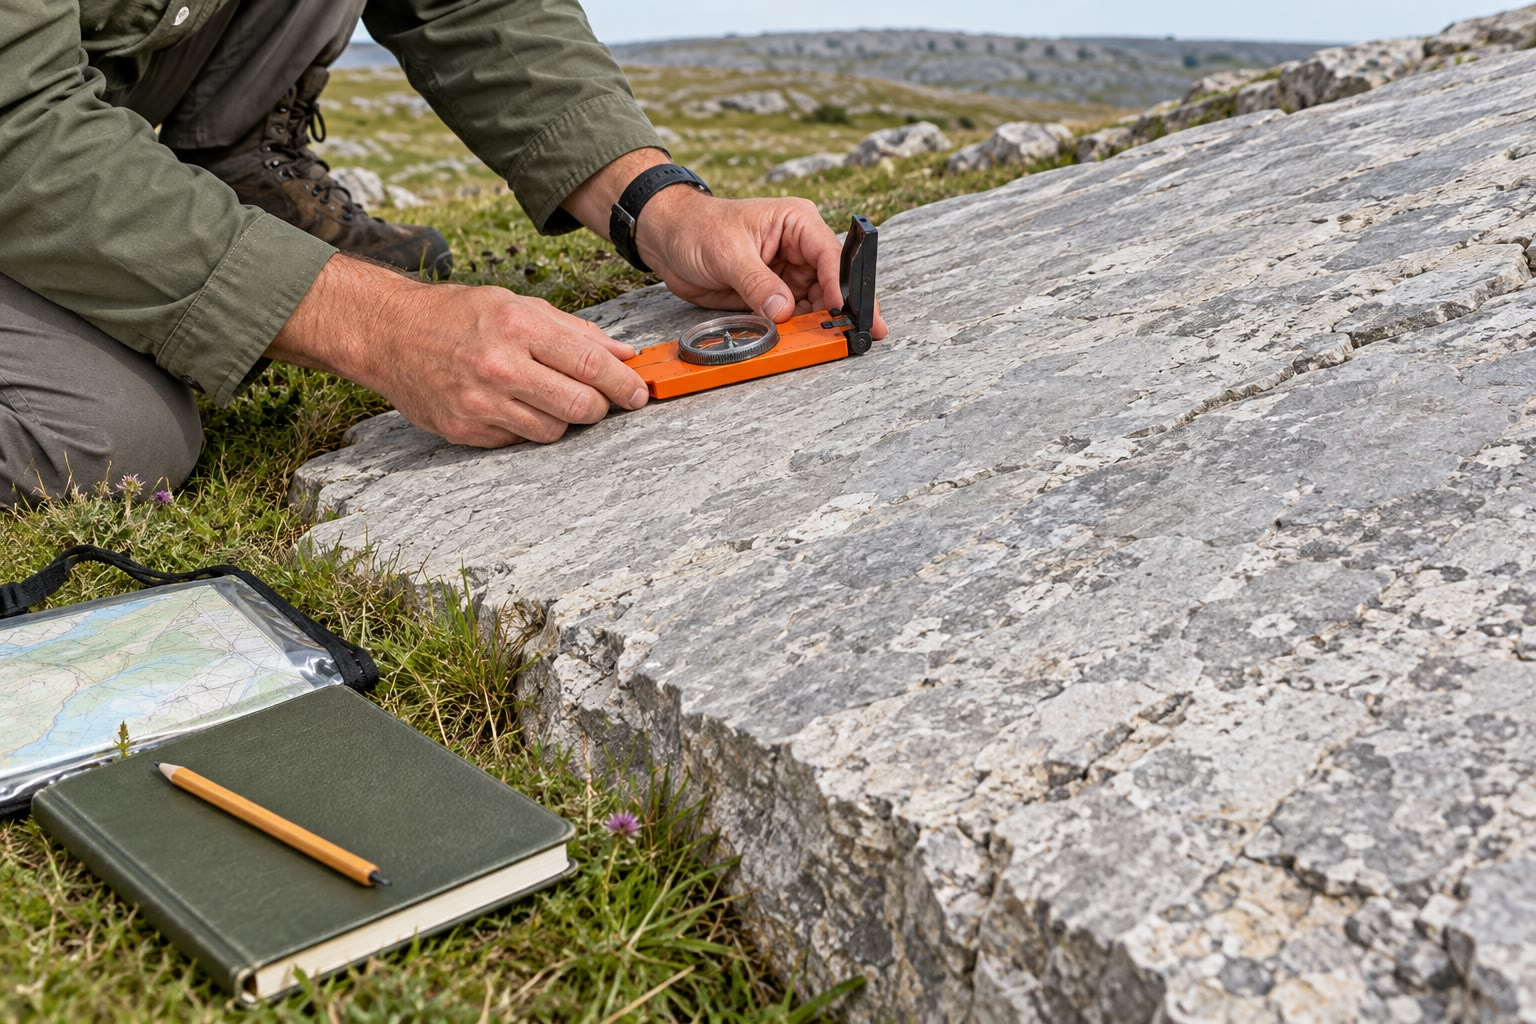
\includegraphics[width=0.6\linewidth]{images/book3/ai/b1-compass-clinometer.jpg}
\end{center}
\end{inthefield}

\begin{history}[Peta geologi pertama sebuah negara]
% ledger: gsl:smith-1815, commons:smith-1815
Juru ukur William Smith, yang menggali kanal dan mengeringkan tanah di Inggris, memperhatikan bahwa setiap lapisan batuan memuat fosilnya sendiri, dalam urutan yang sama di mana pun. Dengan memakai fosil untuk mengenali lapisan-lapisan itu, ia mengikutinya melintasi negeri selama lebih dari lima belas tahun. Petanya, \emph{A Delineation of the Strata of England and Wales, with part of Scotland}, berangka 1 Agustus 1815, dianggap sebagai \omterm{def:b1:geological-maps:geological-map}{peta geologi} pertama dari sebuah negara yang lengkap.
\begin{center}
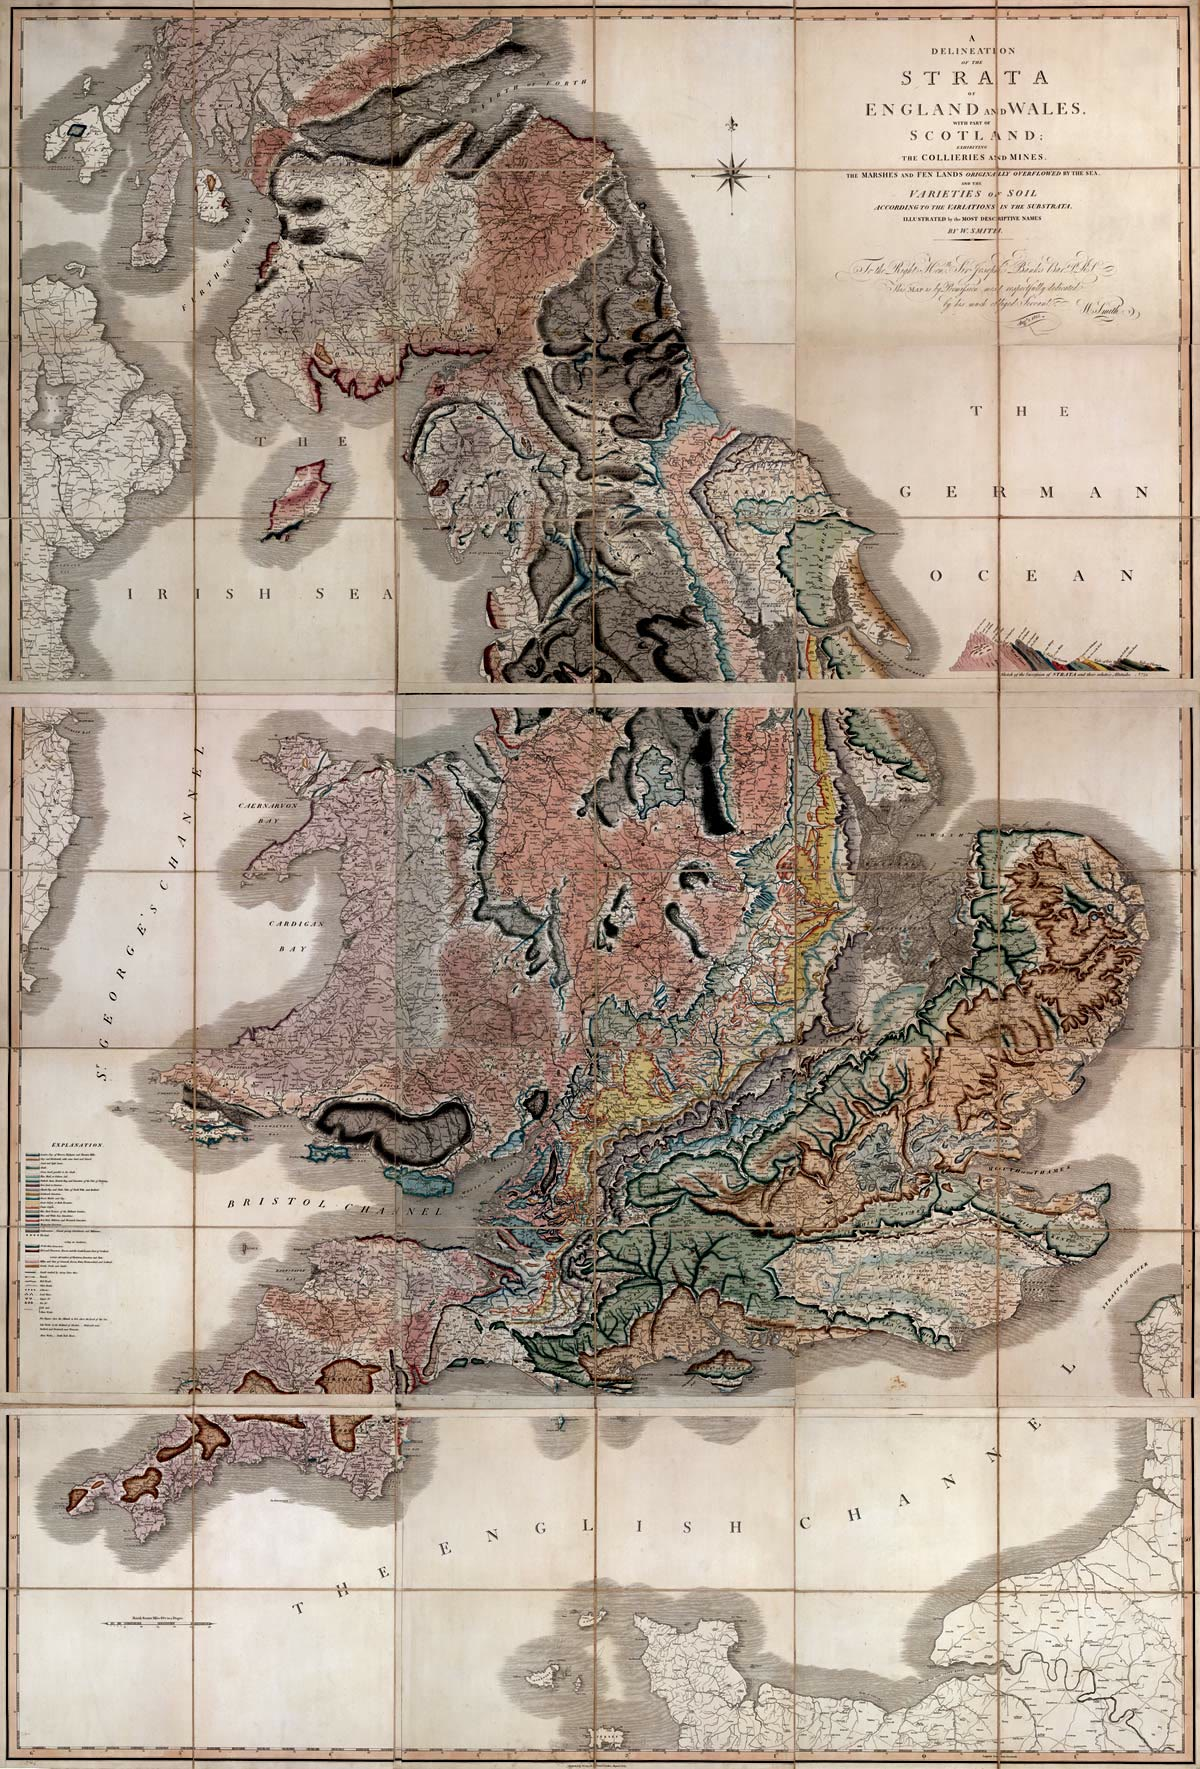
\includegraphics[width=0.36\linewidth]{images/book3/b1-smith-1815-map.jpg}

{\small Peta William Smith tahun 1815 (domain publik).}
\end{center}
\end{history}

\section{Latihan}

\begin{exercise}[$\star$]\label{exo:b1:geological-maps:1}
Definisikan \omterm{def:b1:geological-maps:attitude}{jurus}, \omterm{def:b1:geological-maps:attitude}{kemiringan}, dan \omterm{def:b1:geological-maps:attitude}{arah kemiringan} suatu bidang. Sebuah lapisan memiliki \omterm{def:b1:geological-maps:attitude}{orientasi} $135/40$: nyatakan \omterm{def:b1:geological-maps:attitude}{jurusnya} menurut kaidah tangan kanan dan gambarkan simbol petanya.
\end{exercise}

\begin{exercise}[$\star$]\label{exo:b1:geological-maps:2}
Tulislah persamaan bidang berorientasi $090/30$ yang melalui titik $(0, 0, 500)$, koordinat dalam meter. Pada elevasi berapakah ia berada di $(1000, 0)$ dan di $(0, 1000)$?
\end{exercise}

\begin{exercise}[$\star$]\label{exo:b1:geological-maps:3}
Pada peta, jejak suatu \omterm{def:b1:geological-maps:geological-map}{kontak} mengikuti garis kontur \qty{350}{m} dengan tepat, sepanjang beberapa kilometer bukit dan lembah. Apa yang dapat dikatakan tentang \omterm{def:b1:geological-maps:geological-map}{kontak} itu? Dan jika jejaknya berupa garis lurus yang melintasi bukit dan lembah?
\end{exercise}

\begin{exercise}[$\star$]\label{exo:b1:geological-maps:4}
Pada peta Perbukitan Varden, satuan mana yang tersingkap di inti \omterm{def:b1:geological-maps:fold}{antiklin} di sepanjang sungai, dan satuan mana yang menempati inti \omterm{def:b1:geological-maps:fold}{sinklin}? Jelaskan mengapa dengan prinsip superposisi.
\end{exercise}

\begin{exercise}[$\star\star$]\label{exo:b1:geological-maps:5}
Sebuah \omterm{def:b1:geological-maps:geological-map}{kontak} ditemui pada elevasi $\qty{300}{m}$ di $(0, 0)$, $\qty{300}{m}$ di
$(1000, 0)$ dan $\qty{200}{m}$ di $(0, 500)$ (meter, $x$ ke timur, $y$ ke utara). Tentukan \omterm{def:b1:geological-maps:attitude}{jurus}, \omterm{def:b1:geological-maps:attitude}{arah kemiringan}, dan \omterm{def:b1:geological-maps:attitude}{kemiringannya}, pertama dengan bernalar pada kontur struktur, kemudian dengan \cref{thm:b1:geological-maps:three-point}.
\end{exercise}

\begin{exercise}[$\star\star$]\label{exo:b1:geological-maps:6}
Dasar lembah menurun ke utara sebesar \qty{30}{m} per km. Ke arah mana V \omterm{def:b1:geological-maps:geological-map}{singkapan} suatu \omterm{def:b1:geological-maps:geological-map}{kontak} menunjuk jika \omterm{def:b1:geological-maps:geological-map}{kontak} itu (a) horizontal; (b) miring \ang{20} ke selatan; (c) miring \ang{1} ke utara; (d) miring \ang{20} ke utara? Benarkan dengan \cref{thm:b1:geological-maps:v-rule}.
\end{exercise}

\begin{exercise}[$\star\star$]\label{exo:b1:geological-maps:7}
Dalam keadaan aturan-V, sebuah \omterm{def:b1:geological-maps:geological-map}{kontak} miring ke hilir dengan $a = 0.364$ (\ang{20}) dan dasar lembah menurun dengan $s = 0.03$. Sebuah titik pada sisi lembah \qty{80}{m} lebih tinggi daripada dasar. Berapa jauh ke hulu dari puncak V jejak di titik itu?
\end{exercise}

\begin{exercise}[$\star\star$]\label{exo:b1:geological-maps:8}
\omterm{def:b1:geological-maps:geological-map}{Singkapan} \omterm{def:b1:geological-maps:fold}{antiklin} Varden menutup di sekitar ujung utara intinya. Ke arah mana \omterm{def:b1:geological-maps:fold}{sumbu lipatan} menunjam? Apakah \omterm{def:b1:geological-maps:geological-map}{singkapan} \omterm{def:b1:geological-maps:fold}{sinklin} akan menutup ke utara atau ke selatan?
\end{exercise}

\begin{exercise}[$\star\star$]\label{exo:b1:geological-maps:9}
Pada \omterm{def:b1:geological-maps:geological-map}{peta geologi}, di sepanjang sesar, sisi mana yang menampilkan satuan yang lebih muda di permukaan? Blok mana yang bergerak turun? Periksa terhadap simbol peta.
\end{exercise}

\begin{exercise}[$\star\star\star$]\label{exo:b1:geological-maps:10}
Tunjukkan bahwa dua bidang dengan \omterm{def:b1:geological-maps:attitude}{orientasi} $(\alpha_1, \delta_1)$ dan
$(\alpha_2, \delta_2)$ berpotongan sepanjang garis yang sejajar dengan $\vec n_1 \times \vec n_2$, dengan $\vec n_i = (\tan\delta_i\sin\alpha_i,
\tan\delta_i\cos\alpha_i, 1)$. Terapkan pada bidang $090/30$ dan $270/30$: apakah garisnya, dan \omterm{def:b1:geological-maps:fold}{lipatan} jenis apa yang dibentuk kedua bidang itu?
\end{exercise}

\begin{exercise}[$\star\star\star$]\label{exo:b1:geological-maps:11}
Sebuah gang vertikal berjurus \ang{045} dan tersingkap di titik asal, di dasar lembah pada elevasi \qty{0}{m}. Di mana jejaknya dapat berada di bukit pada \qty{300}{m}? Gang kedua berjurus sama, miring \ang{60} ke tenggara dan juga tersingkap di titik asal. Berapa jauh dari titik asal, dan ke arah mana, jejaknya berada di tanah pada \qty{300}{m}, diukur tegak lurus terhadap \omterm{def:b1:geological-maps:attitude}{jurus}?
\end{exercise}

\begin{exercise}[$\star\star\star$]\label{exo:b1:geological-maps:12}
Dalam \omterm{def:b1:geological-maps:dem}{model elevasi digital} dengan kisi \qty{100}{m}, tanah pada $(x, y)$ dan pada $(x + 100, y)$ berada pada 420 dan \qty{405}{m}, dan pada $(x, y + 100)$ pada \qty{412}{m}. Anggaplah tanah dalam sel itu sebagai bidang, hitunglah \omterm{def:b1:geological-maps:attitude}{kemiringannya} (dalam derajat) dan \omterm{def:b1:spherical-astronomy:horizontal}{azimut} arah ia menghadap (arah menurun lereng).
\end{exercise}

\section{Soal: Menyelesaikan Perbukitan Varden}

\begin{problem}[{Soal akhir pekan --- dari lubang bor dan sebuah peta menuju sumbu lipatan, sesar, dan sejarah suatu wilayah}]
\label{pb:b1:geological-maps:1}
% all data computed in figdata/bachelor-1/varden_maps.py from the region's
% model (figdata/shared/region.py); invented region: exercise data, no ledger
Sebuah perusahaan pengeboran air di Perbukitan Varden mencatat tempat lubang-lubang bornya menemui dasar batu gamping; geolognya juga menentukan lokasi sesar tempat ia memotong tanah. Koordinat dalam meter ke timur dan utara dari sudut barat daya peta; elevasi dalam meter di atas permukaan laut. Bagian I menggunakan \omterm{def:b1:geological-maps:geological-map}{peta geologi} berwarna pada \cref{sec:b1:geological-maps:cut}.

\medskip
\noindent\textbf{Bagian I --- Membaca peta.}
\begin{enumerate}
  \item Daftarkan satuan-satuan wilayah itu dari yang tertua sampai yang termuda.
  \item Satuan-satuan apa yang dipotong sungai, dari barat ke timur?
  \item Satuan apa yang menempati inti \omterm{def:b1:geological-maps:fold}{lipatan} dekat $x = \qty{3.5}{km}$? \omterm{def:b1:geological-maps:fold}{Lipatan} jenis apa itu?
  \item Satuan apa yang menempati inti \omterm{def:b1:geological-maps:fold}{lipatan} dekat $x = \qty{7.5}{km}$? \omterm{def:b1:geological-maps:fold}{Lipatan} jenis apa itu?
  \item Mengapa sekis dan granit hanya tampak di dekat sungai, di inti \omterm{def:b1:geological-maps:fold}{lipatan} pertama?
  \item \omterm{def:b1:geological-maps:geological-map}{Kontak} jenis apa yang memisahkan batu pasir dari granit? Benarkan dari peta.
\end{enumerate}

\medskip
\noindent Lubang-lubang bor (kedalaman $d$ sampai dasar batu gamping, elevasi tanah $z_g$) dan tiga titik F1--F3 tempat sesar memotong bagian atas batuan dasar (F2, di lembah, berada di bawah aluvium tipis yang tidak dipotong sesar):

\begin{omfigure}
\begin{minipage}[c]{0.42\linewidth}
\centering\small
\begin{tabular}{lrrrr}
\hline
 & timur & utara & $z_g$ & $d$ \\
\hline
E1 & 4000 & 6000 & 435 & 261 \\
E2 & 4600 & 7200 & 432 & 428 \\
E3 & 5100 & 6400 & 512 & 586 \\
W1 & 1500 & 6000 & 524 & 669 \\
W2 & 2200 & 7200 & 421 & 459 \\
W3 & 2600 & 5400 & 319 & 209 \\
\hline
 & timur & utara & $z_g$ & \\
\hline
F1 & 4197 & 1000 & 405 & \\
F2 & 5824 & 3500 & 129 & \\
F3 & 7321 & 6500 & 482 & \\
\hline
\end{tabular}
\end{minipage}\hfill
\begin{minipage}[c]{0.56\linewidth}
\centering
\begin{tikzpicture}
\begin{axis}[axis equal image, xmin=0, xmax=10, ymin=0, ymax=8, width=\linewidth,
  tick label style={font=\scriptsize}, xlabel={timur (km)}, ylabel={utara (km)},
  label style={font=\footnotesize}]
\addplot[fill=black!8, draw=black!50, line width=0.3pt, even odd rule] table {figdata/out/shared-region-unit-schist.dat};
\addplot[fill=black!8, draw=black!50, line width=0.3pt, even odd rule] table {figdata/out/shared-region-unit-granite.dat};
\addplot[fill=icsTriassic!20, draw=black!50, line width=0.3pt, even odd rule] table {figdata/out/shared-region-unit-sandstone.dat};
\addplot[fill=icsJurassic!25, draw=black!50, line width=0.3pt, even odd rule] table {figdata/out/shared-region-unit-limestone.dat};
\addplot[fill=icsJurassic!8, draw=black!50, line width=0.3pt, even odd rule] table {figdata/out/shared-region-unit-shale.dat};
\addplot[fill=icsCretaceous!20, draw=black!50, line width=0.3pt, even odd rule] table {figdata/out/shared-region-unit-chalk.dat};
\addplot[fault] table {figdata/out/shared-region-fault.dat};
\addplot[fill=omLithAlluv, draw=black!50, line width=0.3pt, even odd rule] table {figdata/out/shared-region-unit-alluvium.dat};
\addplot[river] table {figdata/out/shared-region-river.dat};
\addplot[only marks, mark=*, mark size=1.6pt] table[x=x_km, y=y_km] {figdata/out/bachelor-1-varden_maps-boreholes.dat};
\addplot[only marks, mark=square*, mark size=1.5pt, omThm] table[x=x_km, y=y_km] {figdata/out/bachelor-1-varden_maps-fault.dat};
\begin{scope}[every node/.style={font=\scriptsize\bfseries, inner sep=1.5pt, fill=white, fill opacity=0.8, text opacity=1}]
  \node[above right] at (axis cs:4,6) {E1};
  \node[above] at (axis cs:4.6,7.2) {E2};
  \node[right] at (axis cs:5.1,6.4) {E3};
  \node[above left] at (axis cs:1.5,6) {W1};
  \node[above] at (axis cs:2.2,7.2) {W2};
  \node[left] at (axis cs:2.6,5.4) {W3};
  \node[left, text=omThm] at (axis cs:4.197,1) {F1};
  \node[left, text=omThm] at (axis cs:5.824,3.5) {F2};
  \node[left, text=omThm] at (axis cs:7.321,6.5) {F3};
\end{scope}
\end{axis}
\end{tikzpicture}
\end{minipage}
\end{omfigure}

\medskip
\noindent\textbf{Bagian II --- Sayap timur.}
\begin{enumerate}[resume]
  \item Hitunglah elevasi dasar batu gamping di E1, E2 dan E3.
  \item Tuliskan vektor $\overrightarrow{E_1E_2}$ dan
        $\overrightarrow{E_1E_3}$.
  \item Hitunglah hasil kali silangnya dan orientasikan ke atas.
  \item Turunkan \omterm{def:b1:geological-maps:attitude}{kemiringan} dasar batu gamping pada sayap timur.
  \item Turunkan \omterm{def:b1:geological-maps:attitude}{arah kemiringannya}, lalu \omterm{def:b1:geological-maps:attitude}{jurusnya} menurut kaidah tangan kanan.
  \item Apakah hasilnya konsisten dengan simbol \omterm{def:b1:geological-maps:attitude}{jurus} dan \omterm{def:b1:geological-maps:attitude}{kemiringan} sayap timur pada peta?
\end{enumerate}

\medskip
\noindent\textbf{Bagian III --- Lipatan.}
\begin{enumerate}[resume]
  \item Hitunglah elevasi dasar batu gamping di W1, W2 dan W3.
  \item Hitunglah normal ke atas $\vec n_W$ pada dasar batu gamping di sayap barat.
  \item Turunkan \omterm{def:b1:geological-maps:attitude}{orientasi} sayap barat.
  \item Hitunglah arah perpotongan kedua sayap, yaitu \omterm{def:b1:geological-maps:fold}{sumbu lipatan}, sebagai $\vec n_E \times \vec n_W$ (dengan $\vec n_E$ dari soal 9).
  \item Berikan \omterm{def:b1:geological-maps:attitude}{jurusnya} (\omterm{def:b1:spherical-astronomy:horizontal}{azimut} proyeksi horizontal sumbu, diambil ke arah menurun) dan penunjamannya (sudutnya di bawah horizontal) dari \omterm{def:b1:geological-maps:fold}{sumbu lipatan}.
  \item Dasar batu pasir berada pada sumbu di \qty{230}{m} tempat sungai memotongnya, dekat $y = \qty{4}{km}$. Berapa lebih rendah ia pada sumbu sejauh \qty{8}{km} ke utara? Apakah ini konsisten dengan soal 3 Bagian I dan dengan penutupan \omterm{def:b1:geological-maps:geological-map}{singkapan}?
\end{enumerate}

\medskip
\noindent\textbf{Bagian IV --- Sesar dan sejarahnya.}
\begin{enumerate}[resume]
  \item Dari F1, F2 dan F3, hitunglah \omterm{def:b1:geological-maps:attitude}{orientasi} sesar.
  \item Di sepanjang sesar, satuan di permukaan pada sisi timur-tenggara lebih muda daripada yang berhadapan dengannya. Blok mana yang bergerak turun? Apakah sesar itu normal atau naik (sungkup)?
  \item Garis lurus dari F1 ke F3 melewati sekitar \qty{200}{m} di sebelah barat F2. Mengapa jejak sesar membelok ke timur-tenggara ketika ia memotong lembah sungai, di F2?
  \item Urutkan: pelipatan; pengendapan kapur; pensesaran; intrusi granit; erosi sebelum batu pasir; pengendapan aluvium.
  \item Kapur berumur 90 juta tahun dan terlipat; aluvium diendapkan dalam 2.58 juta tahun terakhir dan tidak tersesarkan. Di antara umur berapakah pelipatan dan pensesaran terjadi?
  \item Untuk mencapai sesar pada \qty{1000}{m} di bawah permukaan laut di bawah F1, sejauh mana dari F1, dan ke arah mana, sebuah sumur vertikal harus dibor?
\end{enumerate}
\end{problem}
